%----------------------------------------------------------------------------
\chapter{Related work}
\label{cha:relatedwork}
%----------------------------------------------------------------------------

Model-based testing is a mature idea, and it has an extensive literature. Nevertheless the number of the available tools is less than we can expect that. To really take advantage of model-based testing, reliable tools and automation support are required. A usable model-based testing tool has to help in the whole testing process. That means creating and verifying the model, generating test cases, constructing test scripts, adaptors and oracles. Utting, Pretschner and Legeard \cite{taxonomy} defined MBT as testing that relies on models specifying the intended behaviour of the SUT. In reality that would mean restricting MBT to black-box testing, where we can only generate abstract test cases from the behaviour model. That's why Shafique and Labiche defined MBT as a support of software testing activities from a model of the SUT behaviour. We follow this point of view in this paper.

Shafique and Labiche \cite{toolsreview} collected the available tools that rely on state-based models and created a systematic review considering the previously and newly defined criteria.

\begin{description}
	\item[Model-flow criteria] This criterion details the state-based coverage options and applicable to state-based models, which belong to transition-based models. The coverage options can be state, transition, transition-pair, sneak path, all-paths and scenario criteria. The first five are well-known, scenario criteria means, that the test should follow user defined test sequence to pass.
	\item[Script-flow criteria] This criterion refers to interface (function), statement, decision/branch, condition, modified-condition/decision and atomic-condition. They can extend the finite state machine's mechanism. Interfaces refer to the functions which are called on the SUT, the others can serve as guards on transitions.
	\item[Data criteria] This criterion refers to the selection of input values when creating concrete test cases from abstract test cases. The options are one-value, all-values, boundary-values and pair-wise values. By one-value only one concrete test case will be generated for an abstract test case, by all-value all concrete test case will be generated for an abstract test case. Boundary-value means selecting values from a specific range.
	\item[Requirement criteria] It is a binary decision whether a tool supports checking of requirement's satisfaction or not. Requirements are linked to a specific part of the model (e.g.: transition, state).
	\item[Scaffolding criteria] Scaffolding means generating part of a required code. Fully support refers to scaffolding out all needed part of the process, partially support means only a few of them.
\end{description}

\section{GraphWalker}
\label{sec:graphwalker}

The first investigated tool was GraphWalker \cite{graphwalker}, which can create online and offline tests from finite state machines, extended finite state machines or from both of them. The framework is written in Java, the related tools belong to Java world as well. Maven is used to run the tests, TestNG to describe the test cases.

The input model has to be in GraphML format, which is an easy-to-use, highly extendable XML extension for describing graphs. The creators of this software think that UML is too complex, and its functionality is not necessary by software testing, that's why they chose this format. Recommended tool to create GraphML is yED, which is a graphical graph editing software.

After designing the model, test stubs, adaptors and oracles will be generated. The test stub has to be filled with the linking logic with the SUT. While running the tests GraphWalker can use different methods to walk on the state space. For example A* search, shortest path, random path, all permutation. The tests will stop when a certain stop criterion has been satisfied. The stop criteria are state coverage, transition coverage, requirement coverage and time limit.

% secsection graphwalker (end)

\section{PyModel}
\label{sec:pymodel}

PyModel \cite{pymodelarticle}\cite{pymodel} is an open-source MBT testing framework written in Python. It consists three main tools:

\begin{description}
	\item[pma - PyModel Analyzer] It validates the model and creates FSM from it.
    \item[pmg - PyModel Graphics] It generates graphical representation of the FSM.
    \item[pmt - PyModel Tester] It creates online and offline test cases and executes them.
\end{description}

PyModel's test input has to be created by code. The methods will be the transitions in the FSM, states are the defined attributes. It is possible to combine different models in a test. Scenarios supported as well, so user can guide the tests with a given test case sequence. There are two test coverage criteria, state-based and transition-based coverage.

% section pymodel (end)

\section{Conformiq}
\label{sec:conformiq}

Conformiq Designer is one of the most famous, industrial model based testing tool. It is available as a plugin for Eclipse, and in a form of a standalone testing framework. Seeing the success of this software, the design of the software has to be investigated.

The MBT process using Conformiq is identical to the original high level MBT process as it can be seen on Figure~\ref{fig:conformiq_process}.

\begin{figure}[htp]
\centering
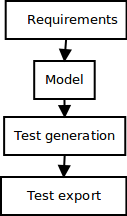
\includegraphics[scale=0.6]{figures/conformiq_process.png}
\caption{MBT process in Conformiq}
\label{fig:conformiq_process}
\end{figure}

\begin{enumerate}
	\item First step is specifying requirements. Conformiq support a huge amount of industrial requirements modelling tool (eg.: IBM Rational, Rhapsody, Sparx Systems Enterprise, ArchitectHP Quality Center, IBM RequisitePro, DOORS), but it contains an own editor too. The defined requirements are traceable through the whole software testing process.
	\item Based on the requirements one has to create the model of the SUT. It can be done with the Conformiq Designer internal model editor using its QML language. The language consists three parts: system block diagrams, which describes the interface of the model (inbound and outbound ports); UML statecharts and Java like action language.
	\item After the modelling phase abstract test cases can be generated. The generation starts with transforming the model to an intermediate Lisp model, that is used during the symbolic execution, which generates the use cases. The user is able to see coverage statistics and a traceability matrix based on the generated test cases.
	\item Abstract test cases have to be exported with so called scripting backend which creates concrete test cases for the SUT.
\end{enumerate}

% section conformiq (end)

\section{GOTCHA}
\label{sec:gotcha}

...

% section gotcha (end)

\section{ParTeG}
\label{sec:parteg}

...

% section parteg (end)

\section{Conclusions}
\label{sec:conclusions}

After investigating five widely used MBT tools, we can draw some consequences.

\begin{table}[htb]
\begin{center}
\begin{tabular}{|l|l|l|l|}
\hline
	\textbf{Name of the tool} & \textbf{Model} & \textbf{Intermediate model} & \textbf{TC generation method}\\\hline
	GraphWalker & UML & GraphML & search based, combinatorial, random\\\hline
	PyModel & FSM + Python & graph & search based\\\hline
	Conformiq & QML & Lisp (CQ$\lambda$) & symbolic execution\\\hline
	GOTCHA & EFSM & graph & BFS, DFS\\\hline
	ParTeG & UML + OCL & graph & DFS\\
\hline
\end{tabular}
\end{center}
\caption{\label{tab:toolssummary} Summary of examined MBT tools}
\end{table}

\begin{itemize}
	\item The tools implement different coverage criteria, but mostly just the easiest ones (state-based and transition based version of structural model coverage criteria). More difficult criteria are avoided, for example data coverage, requirement-based and fault-based criteria and transition pairs coverage from structural coverage criteria.
	\item Script-flow criteria are rarely used techniques. Only a few tools support guards on transitions or use scripts for example to give control information of the SUT.
	\item Scaffolding solutions of the tools are incomplete. Fully automatic generation of test adaptors, oracles are seldom supported.
	\item Regression tests are not supported.
	\item Creators of these tools either try to use an UML like model or FSM (EFSM). FSM models are low level representations of the SUT, so implementing search based algorithms and graph traversal algorithms are relatively easy. When tools using UML model with graph intermediate model, they can not support complex UML state chart elements, such as orthogonal regions.
	\item The intermediate model is just always some kind of graph representations, because the test case generation algorithms are the easiest to implement using graph models (search based test case generation, coverage criteria).
	\item Important thing to note, that the most successful tools use symbolic execution and it can handle the most complex models.
\end{itemize}

% section conclusions (end)

% chapter relatedwork (end)